\documentclass[10pt]{amsart}
\usepackage[margin=1.0in]{geometry}                % See geometry.pdf to learn the layout options. There are lots.
\geometry{letterpaper}                   % ... or a4paper or a5paper or ... 
%\geometry{landscape}                % Activate for for rotated page geometry
%\usepackage[parfill]{parskip}    % Activate to begin paragraphs with an empty line rather than an indent
\usepackage{graphicx}
\usepackage{amssymb}
\usepackage{epstopdf}
\usepackage{enumerate}
\DeclareGraphicsRule{.tif}{png}{.png}{`convert #1 `dirname #1`/`basename #1 .tif`.png}
\setlength{\parindent}{0in} % no paragraph indent

\usepackage{fancyhdr}
\pagestyle{fancy}
\lhead{\footnotesize \parbox{11cm}{The Effect of the NSA Leaks on Tech Stock Volatility} }
\rhead{\footnotesize \parbox{11cm}{} }

\title{The Effect of the NSA Leaks on Tech Stock Volatility - Max Scheiber and Ruslan Zagatskiy}
\date{12.09.2013}

\begin{document}
\maketitle
\section{Preamble}
On June 6th, 2013, Edward Snowden revealed through the British newspaper, \textit{The Guardian}, that the National Security Agency (NSA) can easily extract personal customer data from America's largest tech companies, spanning from email to audio chats. More NSA leaks were released throughout summer 2013.

\section{Question}
\textbf{Did these leaks change the volatility of relevant tech stocks, either in the short term or long run?}

\section{Data}
We explored three main dates. The original leaks happened on \textbf{June 6th, 2013}. \textit{The Guardian} released a second set of leaks on \textbf{June 20th}, and they published a video interview with Snowden on \textbf{July 8th}. \\

The four companies examined were Google (GOOG), Apple (AAPL), Microsoft (MSFT), and Facebook (FB). These were the four companies highlighted in the NSA slide deck that detailed the program and which companies were involved.

\section{Analysis}
\subsection{January to July}
We ran a $GARCH(1,1)$, which confirmed that the tech sector had heteroskedastic returns over the period. Makes sense.

\centerline{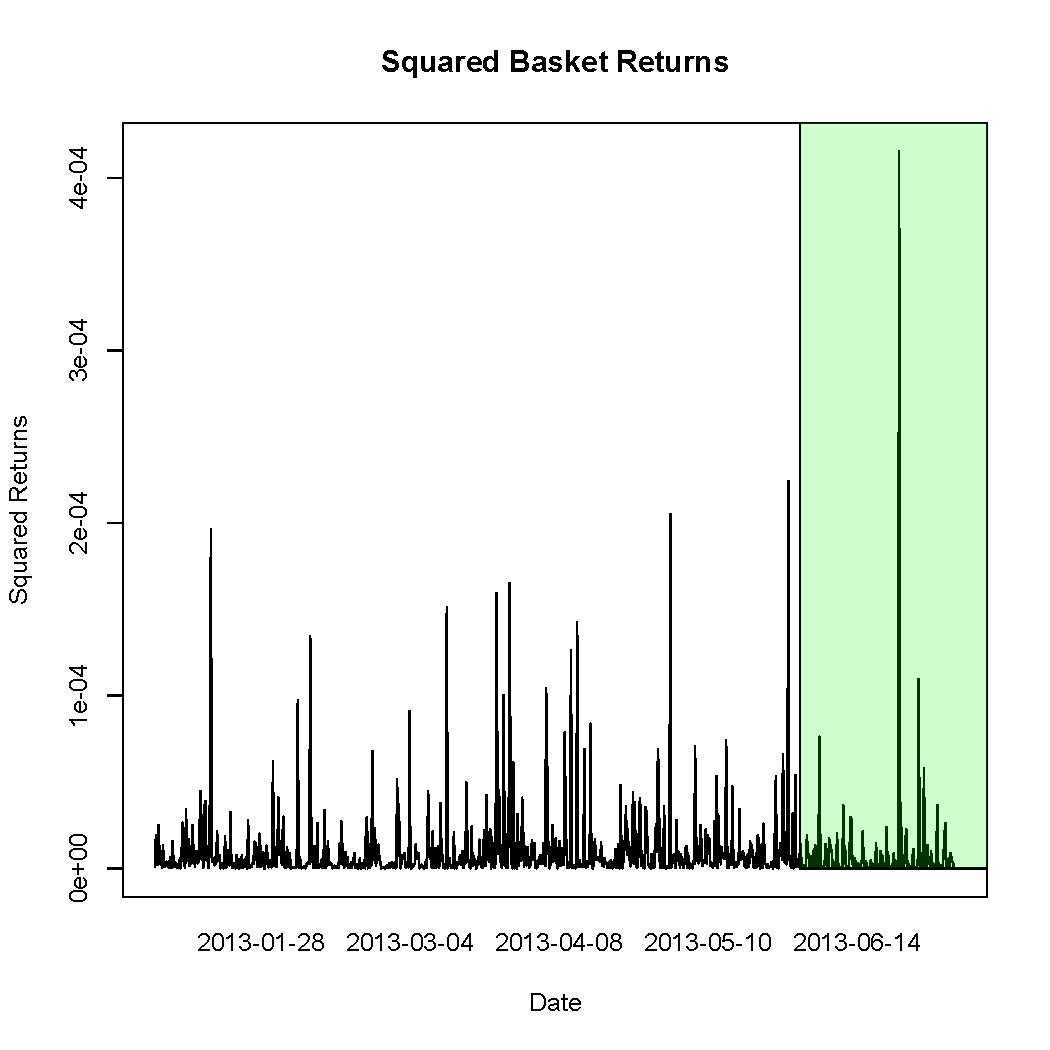
\includegraphics[scale=0.45]{basket_sq_returns_12_08.pdf}}

\subsection{June - significant in short run}
There appears to be heteroskedasticity in the month of June, confirmed via a $GARCH(1,1)$. We ran an OLS regression with indicator variables for June 6-8 and June 20-22 two of our dates of interest. Only the change in volatility during June 20-22 was statistically significant - and only in the short term (June), not medium term (June-July) or long term (January-July).

\newpage

\subsection{July - not significant}
We see a huge spike in volatility around July 20th, but this doesn't correspond with any NSA news. It's likely from quarterly earnings reports - GOOG and MSFT on the 18th, AAPL and FB on the 24th.

\centerline{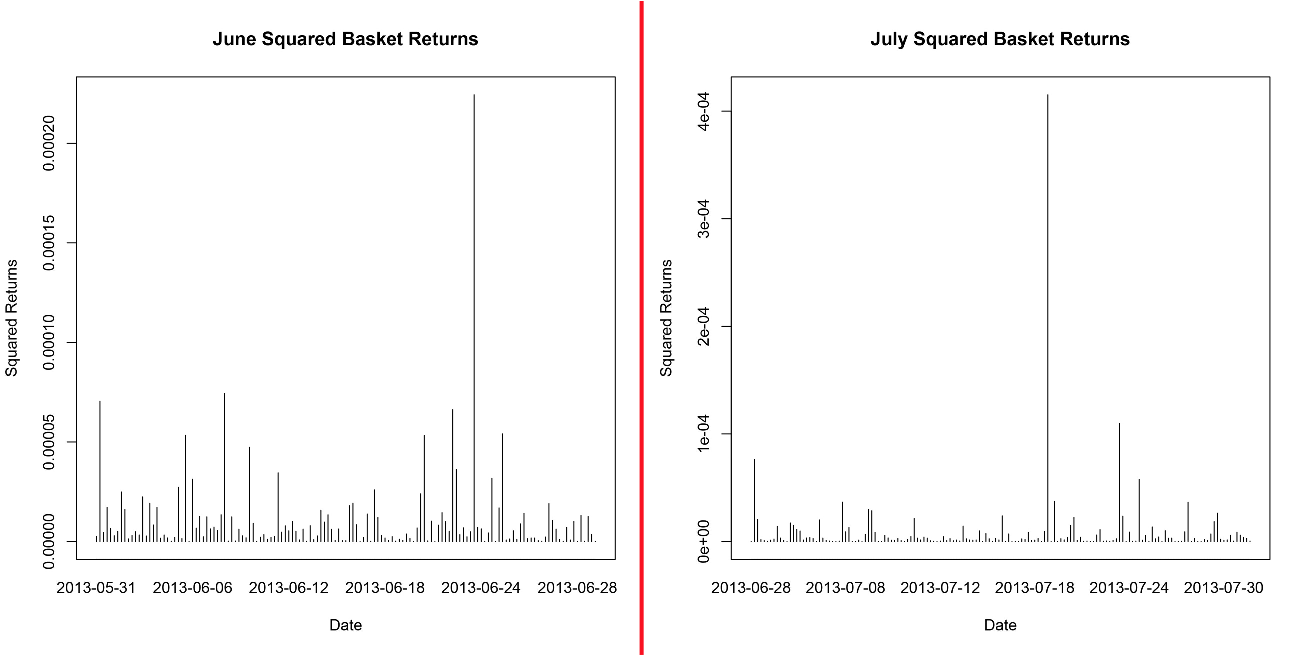
\includegraphics[scale=0.7]{june+july_squared_ret.pdf}}

\subsection{Volume Analysis}
We examined trade volume as well and found results that perfectly mirror those of our volatility analysis. \\

\centerline{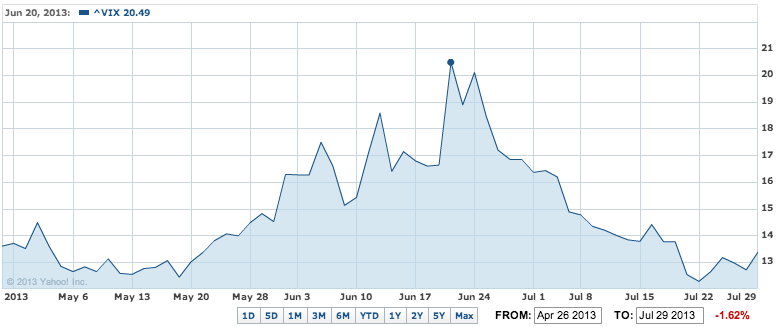
\includegraphics[scale=0.5]{vix_june_20.png}}

\subsection{Full Market Analysis - VIX confirms our intuition}
The VIX, an ETF for the S\&P 500, spiked in volatility on June 20th. The NSA leak was the biggest piece of news on that day. The Fed announced the possibility of reducing its bond buyback program as well. However, we looked at other spikes of similar magnitude on the VIX's volatility, and neither related to the Federal Reserve's monetary policy.

\section{Answer}
If the NSA leaks have changed how we view the world, the market doesn't really reflect that. There was increased volatility in response to one of the leaks, which may have just been some large institutional investor unloading shares. Moreover, this volatility only persisted for a couple of days. \textbf{The NSA leaks affected short-term volatility in one instance but had no long-term effect whatsoever.}

\end{document}  